% !TeX program = xelatex
% 笔记模板：建议使用 XeLaTeX 编译，文件编码保持为 UTF-8。

\documentclass[UTF8,a4paper,11pt]{ctexart}
\usepackage{preamble}
\usepackage{draftwatermark}

\SetWatermarkText{NJUPT}
\SetWatermarkScale{0.5}
\SetWatermarkLightness{0.9}

% 文档信息
\newcommand{\noteheader}{波束成形}
\title{\heiti \noteheader}
\author{黄子恒}
\date{\today}

\begin{document}

\maketitle

\begin{infobox}{Info}
\begin{tabular}{>{\bfseries}p{3cm}p{10cm}}
时间 & 2026.6.28 - 2026.7.10 （第二次组会）\\
内容 & 均匀线阵，均匀面阵，均匀圆阵，均匀圆环阵原理分析与仿真 \\
\end{tabular}
\end{infobox}

\tableofcontents
\newpage

\section{均匀圆阵 UCA}

\begin{figure}[htbp]
\centering
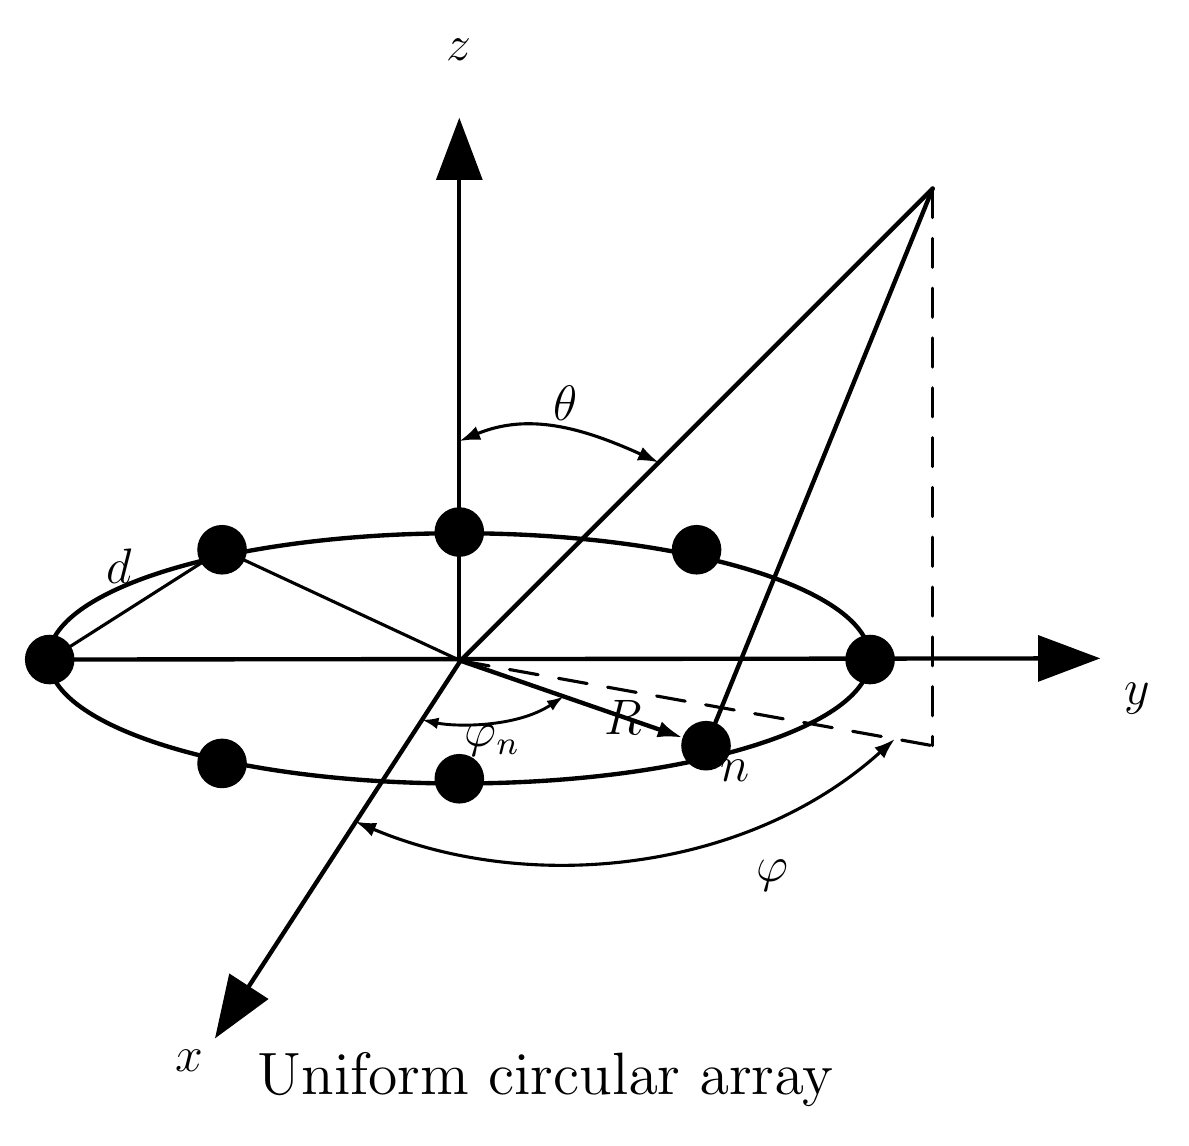
\includegraphics[width=0.85\textwidth]{figures/均匀圆阵示意图.png}
\caption{均匀圆阵的几何结构示意图}
\label{fig:uca-geometry}
\end{figure}

\vspace{1cm}

\textbf{\large 公式推导：}

Tips：\(\theta\) : the elevation plane ，\(\varphi \) : the azimuth
plane

\[
\varphi_n = \frac{2\pi n}{N}, \quad n = 0, 1, \dots, N-1
\]

\[
\mathbf{r}_n = 
\begin{pmatrix}
  R \cdot \cos\varphi_n ,\
  R \cdot \sin\varphi_n ,\
  0
\end{pmatrix}
\]

\[
\mathbf{u}(\varphi, \theta) = 
\begin{pmatrix}
  \cos\varphi \cdot \sin\theta ,\
  \sin\varphi \cdot \sin\theta ,\
  \cos\theta
\end{pmatrix}
\]

\textbf{阵元在观察方向上的投影:}

\[
\begin{aligned}
  \mathbf{r}_n \cdot \mathbf{u}
  &= R\cos\varphi_n \cdot \cos\varphi\sin\theta
  + R\sin\varphi_n \cdot \sin\varphi\sin\theta
  + 0 \cdot \cos\theta\\
  &= R\sin\theta \cdot (\cos\varphi_n\cos\varphi + \sin\varphi_n\sin\varphi)\\
  &= R\sin\theta \cdot \cos(\varphi - \varphi_n)
\end{aligned}
\]

即\texttt{阵元n}与圆心的波程差。
\vspace{10pt}

\textbf{The array factor:}

\[
F(\varphi, \theta) = \sum_{n=0}^{N-1} A_n \cdot e^{j \cdot \bigl[\alpha_n - k \cdot R \cdot \sin\theta \cdot \cos(\varphi - \varphi_n)\bigr]}
\]

其中：

\[
\alpha_n = k \cdot R \cdot \sin\theta_0 \cdot \cos(\varphi_0 - \varphi_n) , k = \frac{2\pi}{\lambda}
\]

\vspace{1cm}
\textbf{\large 仿真文件：}

\texttt{uca\_3d\_pattern.m}



\section{均匀圆环阵 UCCA}

\begin{figure}[htbp]
\centering
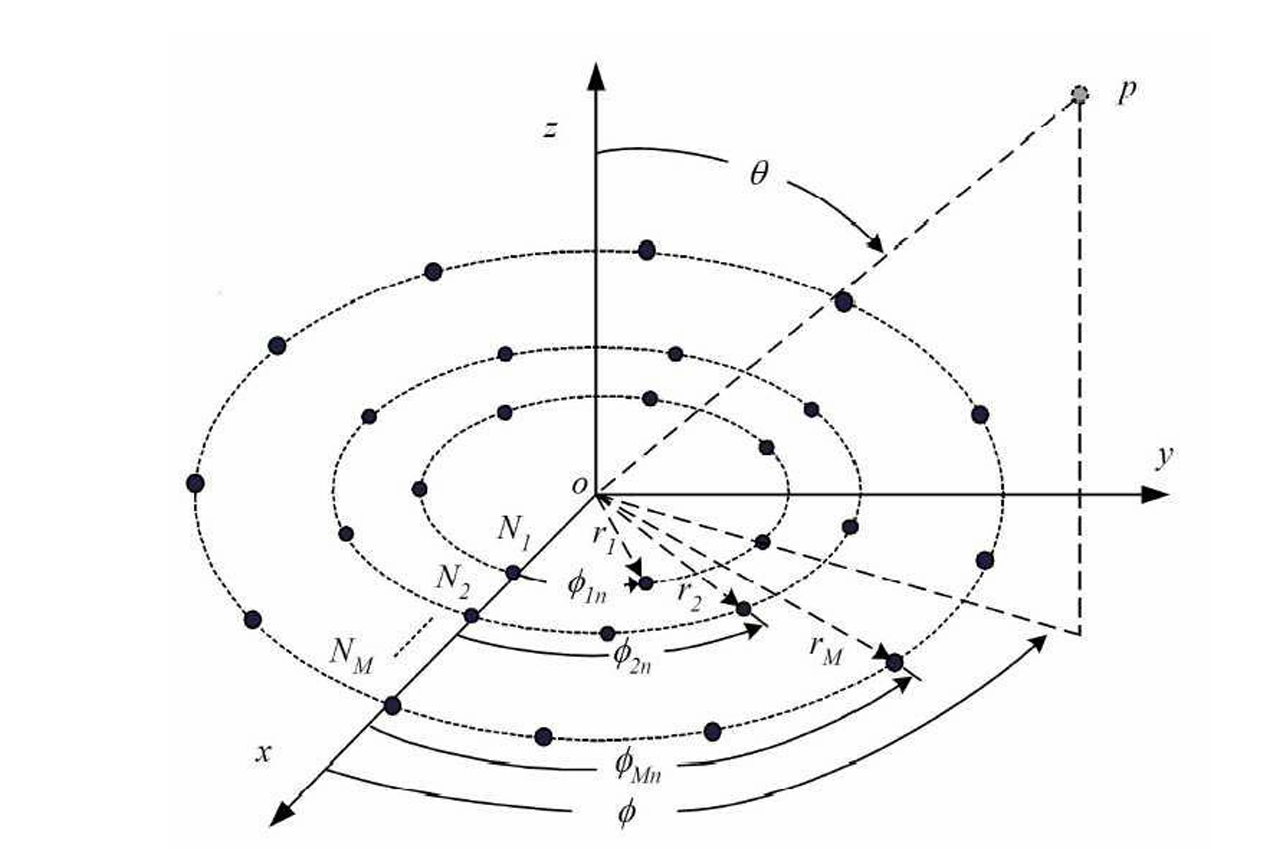
\includegraphics[width=0.85\textwidth]{figures/均匀圆环阵示意图.png}
\caption{均匀圆环阵的几何结构示意图}
\label{fig:ucca-geometry}
\end{figure}

\vspace{1cm}
\textbf{\large 公式推导：}

\[
F(\varphi, \theta) = 1 + \sum_{i=1}^{M} \sum_{j=1}^{N_i} A_{ij} \cdot e^{j \bigl[\alpha_{ij} - k \cdot r_i  \cdot \sin \theta \cos(\varphi - \varphi_{ij}) \bigr]}
\]

其中：

\[
\alpha_{ij} = k \cdot r_i \cdot \sin\theta_0 \cdot \cos(\varphi_0 - \varphi_{ij})
\]

\[
\varphi_{ij} = \frac{2\pi(j - 1)}{N_i}, j = 1,2, \cdots, N_i;
\]

\vspace{1cm}
\textbf{\large 仿真文件：}

\texttt{ucca\_3d\_pattern.m}


\section{均匀线阵 ULA}

\begin{figure}[htbp]
\centering
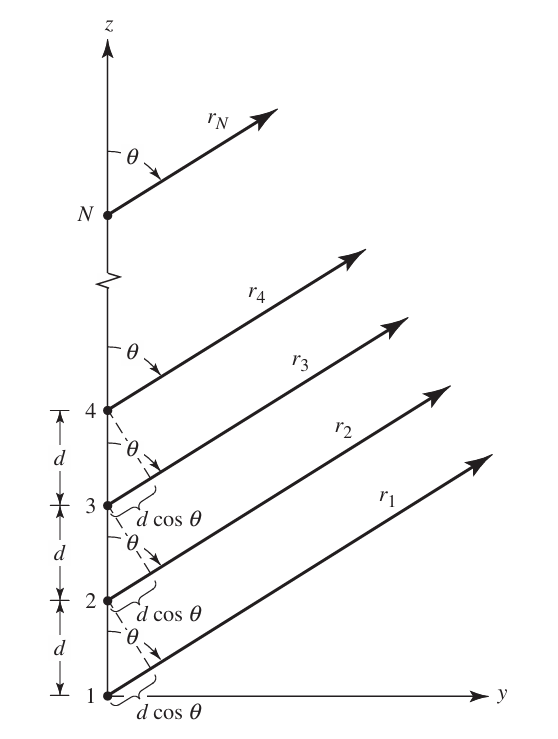
\includegraphics[width=0.6\textwidth]{figures/均匀线阵示意图.png}
\caption{均匀线阵的几何结构示意图}
\label{fig:ula-geometry}
\end{figure}

\vspace{1cm}
\textbf{\large 公式推导：}

相邻两阵元之间的相位差：\texttt{the\ array\ phase\ function}

\[
\psi = kd\cos\theta + \alpha
\]

\textbf{The array factor }(所有阵元振幅相同为1):

\[
\begin{aligned}
AF &= \sum_{n=0}^{N-1} e^{j n( k \cdot d \cdot \cos\theta + \alpha)}
   = \sum_{n=0}^{N-1} e^{j n \psi} \\
   &\xlongequal{\text{等比数列求和}} \frac{e^{j N \psi} - 1}{e^{j \psi} - 1} \\
   &= \frac{e^{j \frac{N}{2} \psi} ( e^{j \frac{N}{2} \psi} - e^{-j \frac{N}{2} \psi})}
          {e^{j \frac{\psi}{2}} (e^{j \frac{\psi}{2}} - e^{-j \frac{\psi}{2}})} \\
   &= e^{j (N-1)\frac{\psi}{2}} \cdot \frac{\sin(\frac{N\psi}{2})}{\sin(\frac{\psi}{2})}
\end{aligned}
\]

The array factor after phase shift and normalization becomes:

\[
AF = \frac{1}{N} \cdot \frac{\sin(\frac{N\psi}{2})}{\sin(\frac{\psi}{2})}
\]

\vspace{1cm}
\textbf{仿真文件：}

\texttt{ula\_polar\_pattern.m}


\section{均匀面阵 UPA}



\begin{figure}[htbp]
\centering
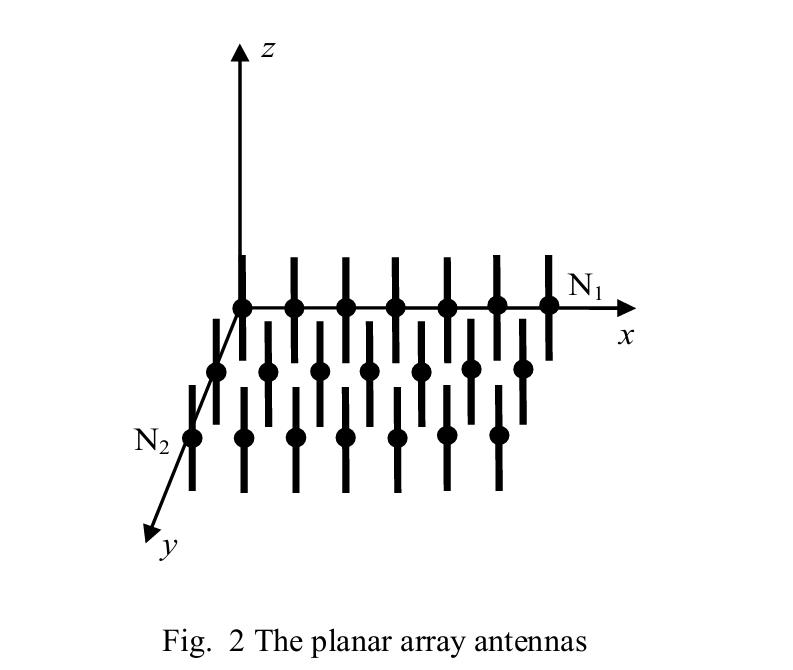
\includegraphics[width=0.5\textwidth]{figures/均匀二维面阵示意图.png}
\caption{均匀二维面阵的几何结构示意图}
\label{fig:upa-2d-geometry}
\end{figure}

\vspace{1cm}
\textbf{\large 公式推导}：

\[
\mathbf{r}_{m,n} = 
\begin{pmatrix}
  m d_x ,\
  n d_y ,\
  0
\end{pmatrix}
\]

\[
\mathbf{u}(\varphi, \theta) = 
\begin{pmatrix}
  \cos\varphi \cdot \sin\theta ,\
  \sin\varphi \cdot \sin\theta ,\
  \cos\theta
\end{pmatrix}
\]

阵元\texttt{（m,n）}与原点的波程差：

\[
\begin{aligned}
  \mathbf{r}_{m,n} \cdot \mathbf{u}
  = m d_x \cdot \cos\varphi\sin\theta
  + n d_y \cdot \sin\varphi\sin\theta
  + 0 \cdot \cos\theta
\end{aligned}
\]

阵元\texttt{（m,n）}的几何相位 (原点相位为0)：

\[
m \cdot(k \cdot d_x \cos\varphi \sin\theta  ) + n \cdot(k \cdot d_y \sin\varphi \sin\theta  )
\]

令：

\[
\begin{aligned}
\psi_x &= kd_x \cos\varphi \sin\theta  + \alpha_x \\
\psi_y &= kd_y \sin\varphi \sin\theta  + \alpha_y
\end{aligned}
\]

其中：

\[
\begin{aligned}
\alpha_x &= -kd_x \sin\theta_0 \cos\phi_0 \\
\alpha_y &= -kd_y \sin\theta_0 \sin\phi_0 
\end{aligned}
\]

\textbf{The array factor }(所有阵元振幅相同为1):

\[
\begin{aligned}
AF &= \sum_{m=0}^{N_1-1} \sum_{n=0}^{N_2-1} e^{j(m\psi_x + n\psi_y)}
   = \sum_{m=0}^{N_1-1} \sum_{n=0}^{N_2-1} e^{j m \psi_x} \cdot e^{j n \psi_y} \\
   &= \left( \sum_{m=0}^{N_1-1} e^{jm\psi_x} \right) \left( \sum_{n=0}^{N_2-1} e^{jn\psi_y} \right)
   = AF_x \cdot AF_y \\
   &= \frac{\sin\left(\frac{N_1 \psi_x}{2}\right)}{N_1 \sin\left(\frac{\psi_x}{2}\right)}
      \cdot \frac{\sin\left(\frac{N_2 \psi_y}{2}\right)}{N_2 \sin\left(\frac{\psi_y}{2}\right)}
\end{aligned}
\]

\vspace{1cm}
\textbf{仿真文件：}

\texttt{upa\_3d\_pattern.m}


\vspace{1cm}
\textbf{\large 3维阵列：}
\vspace{1cm}

\begin{figure}[htbp]
\centering
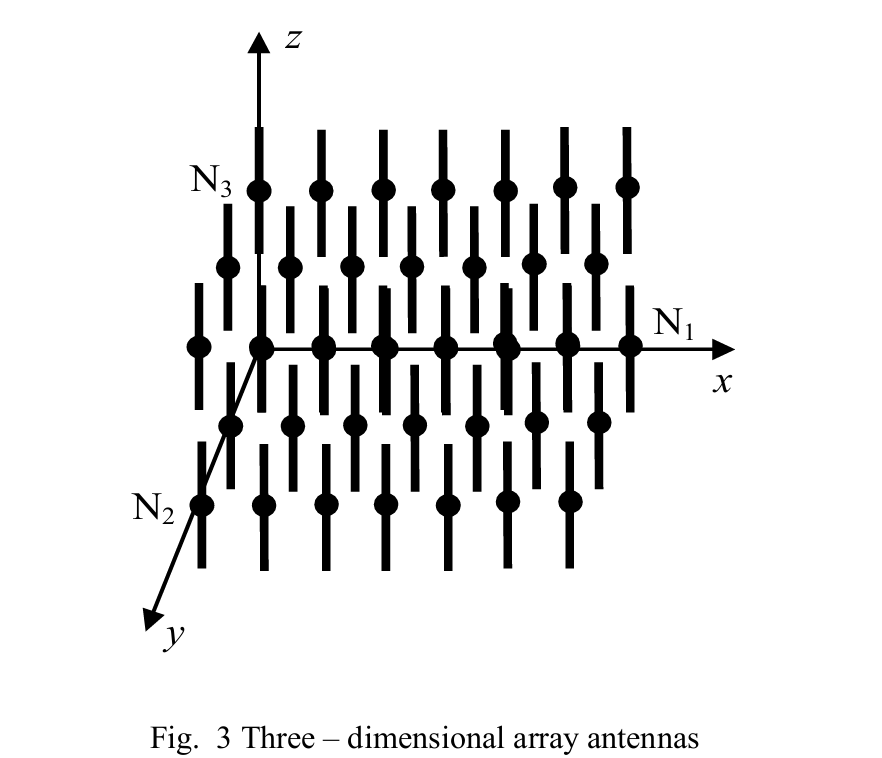
\includegraphics[width=0.5\textwidth]{figures/均匀三维面阵示意图.png}
\caption{均匀三维面阵的几何结构示意图}
\label{fig:upa-3d-geometry}
\end{figure}

\textbf{同理可得：}

\[
\begin{aligned}
\psi_x &= kd_x \sin\theta \cos\varphi + \alpha_x \\
\psi_y &= kd_y \sin\theta \sin\varphi + \alpha_y \\
\psi_z &= kd_z \cos\theta + \alpha_z
\end{aligned}
\]

其中：
\[
\begin{aligned}
\alpha_x &= -kd_x \sin\theta_0 \cos\phi_0 \\
\alpha_y &= -kd_y \sin\theta_0 \sin\phi_0 \\
\alpha_z &= -kd_z \cos\theta_0
\end{aligned}
\]

\textbf{The array factor }(所有阵元振幅相同为1):

\[
\begin{aligned}
AF &= AF_x \cdot AF_y \cdot AF_z = \frac{\sin\left(\frac{N_1 \psi_x}{2}\right)}{N_1 \sin\left(\frac{\psi_x}{2}\right)} \cdot
   \frac{\sin\left(\frac{N_2 \psi_y}{2}\right)}{N_2 \sin\left(\frac{\psi_y}{2}\right)} \cdot
   \frac{\sin\left(\frac{N_3 \psi_z}{2}\right)}{N_3 \sin\left(\frac{\psi_z}{2}\right)}
\end{aligned}
\]

\vspace{1cm}
\textbf{仿真文件：}

\texttt{uva\_3d\_pattern.m}


\section{半波偶极子的归一化方向图函数：}
\[
F(\theta) = \frac{\cos\left( \frac{\pi}{2} \cos\theta \right)}{\sin\theta}
\]

\begin{figure}[htbp]
\centering
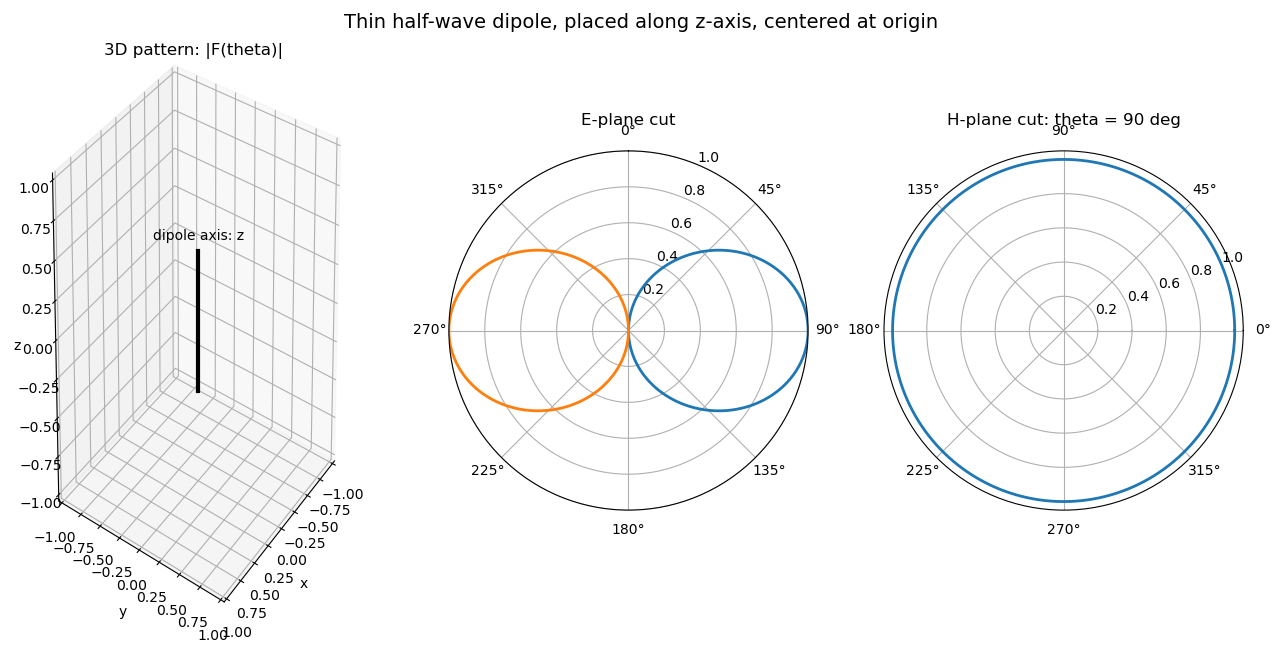
\includegraphics[width=0.85\textwidth]{figures/半波偶极子归一化方向图函数.png}
\caption{半波偶极子的归一化方向图函数}
\label{fig:dipole-pattern}
\end{figure}

\end{document}
